\documentclass{article}
\usepackage[utf8]{inputenc}
\usepackage{graphicx}
\usepackage[margin=1in]{geometry}
\usepackage{float}
\usepackage{amsmath}
\usepackage{epstopdf}
\usepackage{wrapfig}

\title{Final Project: Tunable Ring Oscillator}
\author{Dan Kearney and Theo Thompson}
\date{May 9, 2013}

\begin{document}
\maketitle

\section*{Executive Summary}

For our final project we explored the tunable ring oscillator.  We constructed a three-inverter ring oscillator that we made tunable by wrapping one inverter in a current starver.  We simulated the same circuit and compared the simulated results to the experimental data.

\subsection*{Ring Oscillator Operation}

The ring oscillator, at its core, is an odd number of inverters connected in a circle.  Using logic gates, this can be expressed quite simply in Figure \ref{simpleSchem}.

\begin{figure}[H]
\centering
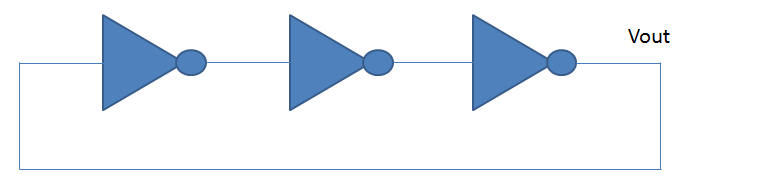
\includegraphics[scale=.4]{simpleSchem.png}
\caption{A logic gate representation of a simple ring oscillator.}
\label{simpleSchem}
\end{figure}

Assuming an ideal inverter with a propagation delay (i.e., that there is a transistion period, but the output is never between 0 and 1), this circuit would produce square waves as each inverter continuously transistions from a 1 to a 0 state and back again.  This is only an approximation for the reality of this situation, and the real circuit produces a waveform with curvature.

We used the circuit in Figure \ref{ring} as the inspiration for our basic ring oscillator.  If we directly connect the output of an inverter to the input of another one, the circuit transitions from 1 to 0 very quickly, slowed only by the node capacitance of the inverters.  The RC circuit between each inverter slows that transition, so changing that time constant changes the frequency of oscillation.  Other factors - such as the transistors' parameters - also affect this frequency by changing the current response of the circuit.  For our RC circuit, we chose a 1 nF capacitor and a 1 $k\Omega$ resistor to give us a time constant of 1 $\mu s$, which meant that we could expect our oscillations to happen, at most, at 1 MHz, since it will take around $1 \mu s$ for the RC circuit's output will go from 0V to a little over 50\% of the rail for the best-case scenario.  In reality, we expect the transition to happen much slower, because the RC circuit's input is not a constant, but a slowly increasing voltage coming from another inverter. 

\begin{figure}[H]
\centering
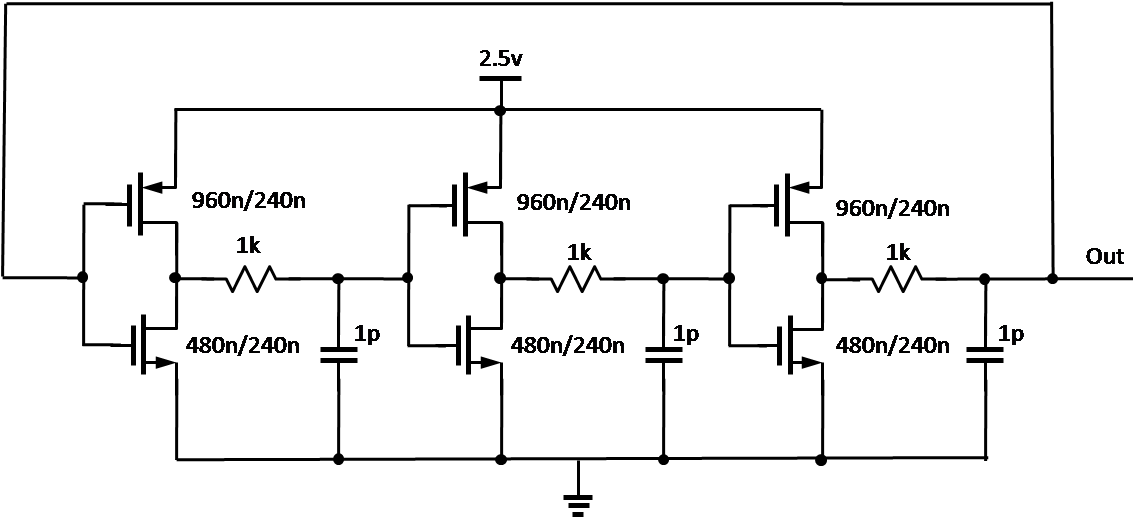
\includegraphics[scale=.5]{ringOsc.png}
\caption{The basic, non-current-starved ring oscillator circuit that we used to build part of our final circuit.  \emph{Source: wikipedia commons.}}
\label{ring}
\end{figure}

The next part of the circuit was the current ``starver'', which is essentially a current mirror that limits the current through one inverter to make it transition more slowly. By setting the bias voltage of the starver, one can tune the frequency of the oscillator.  This slower tranisition makes the next inverter transition more slowly, which makes the next inverter transition at the same rate. As a result, they all stay on the same frequency. A current starver is in Figure \ref{starver}. 
					
\begin{figure}[H]	
\centering			
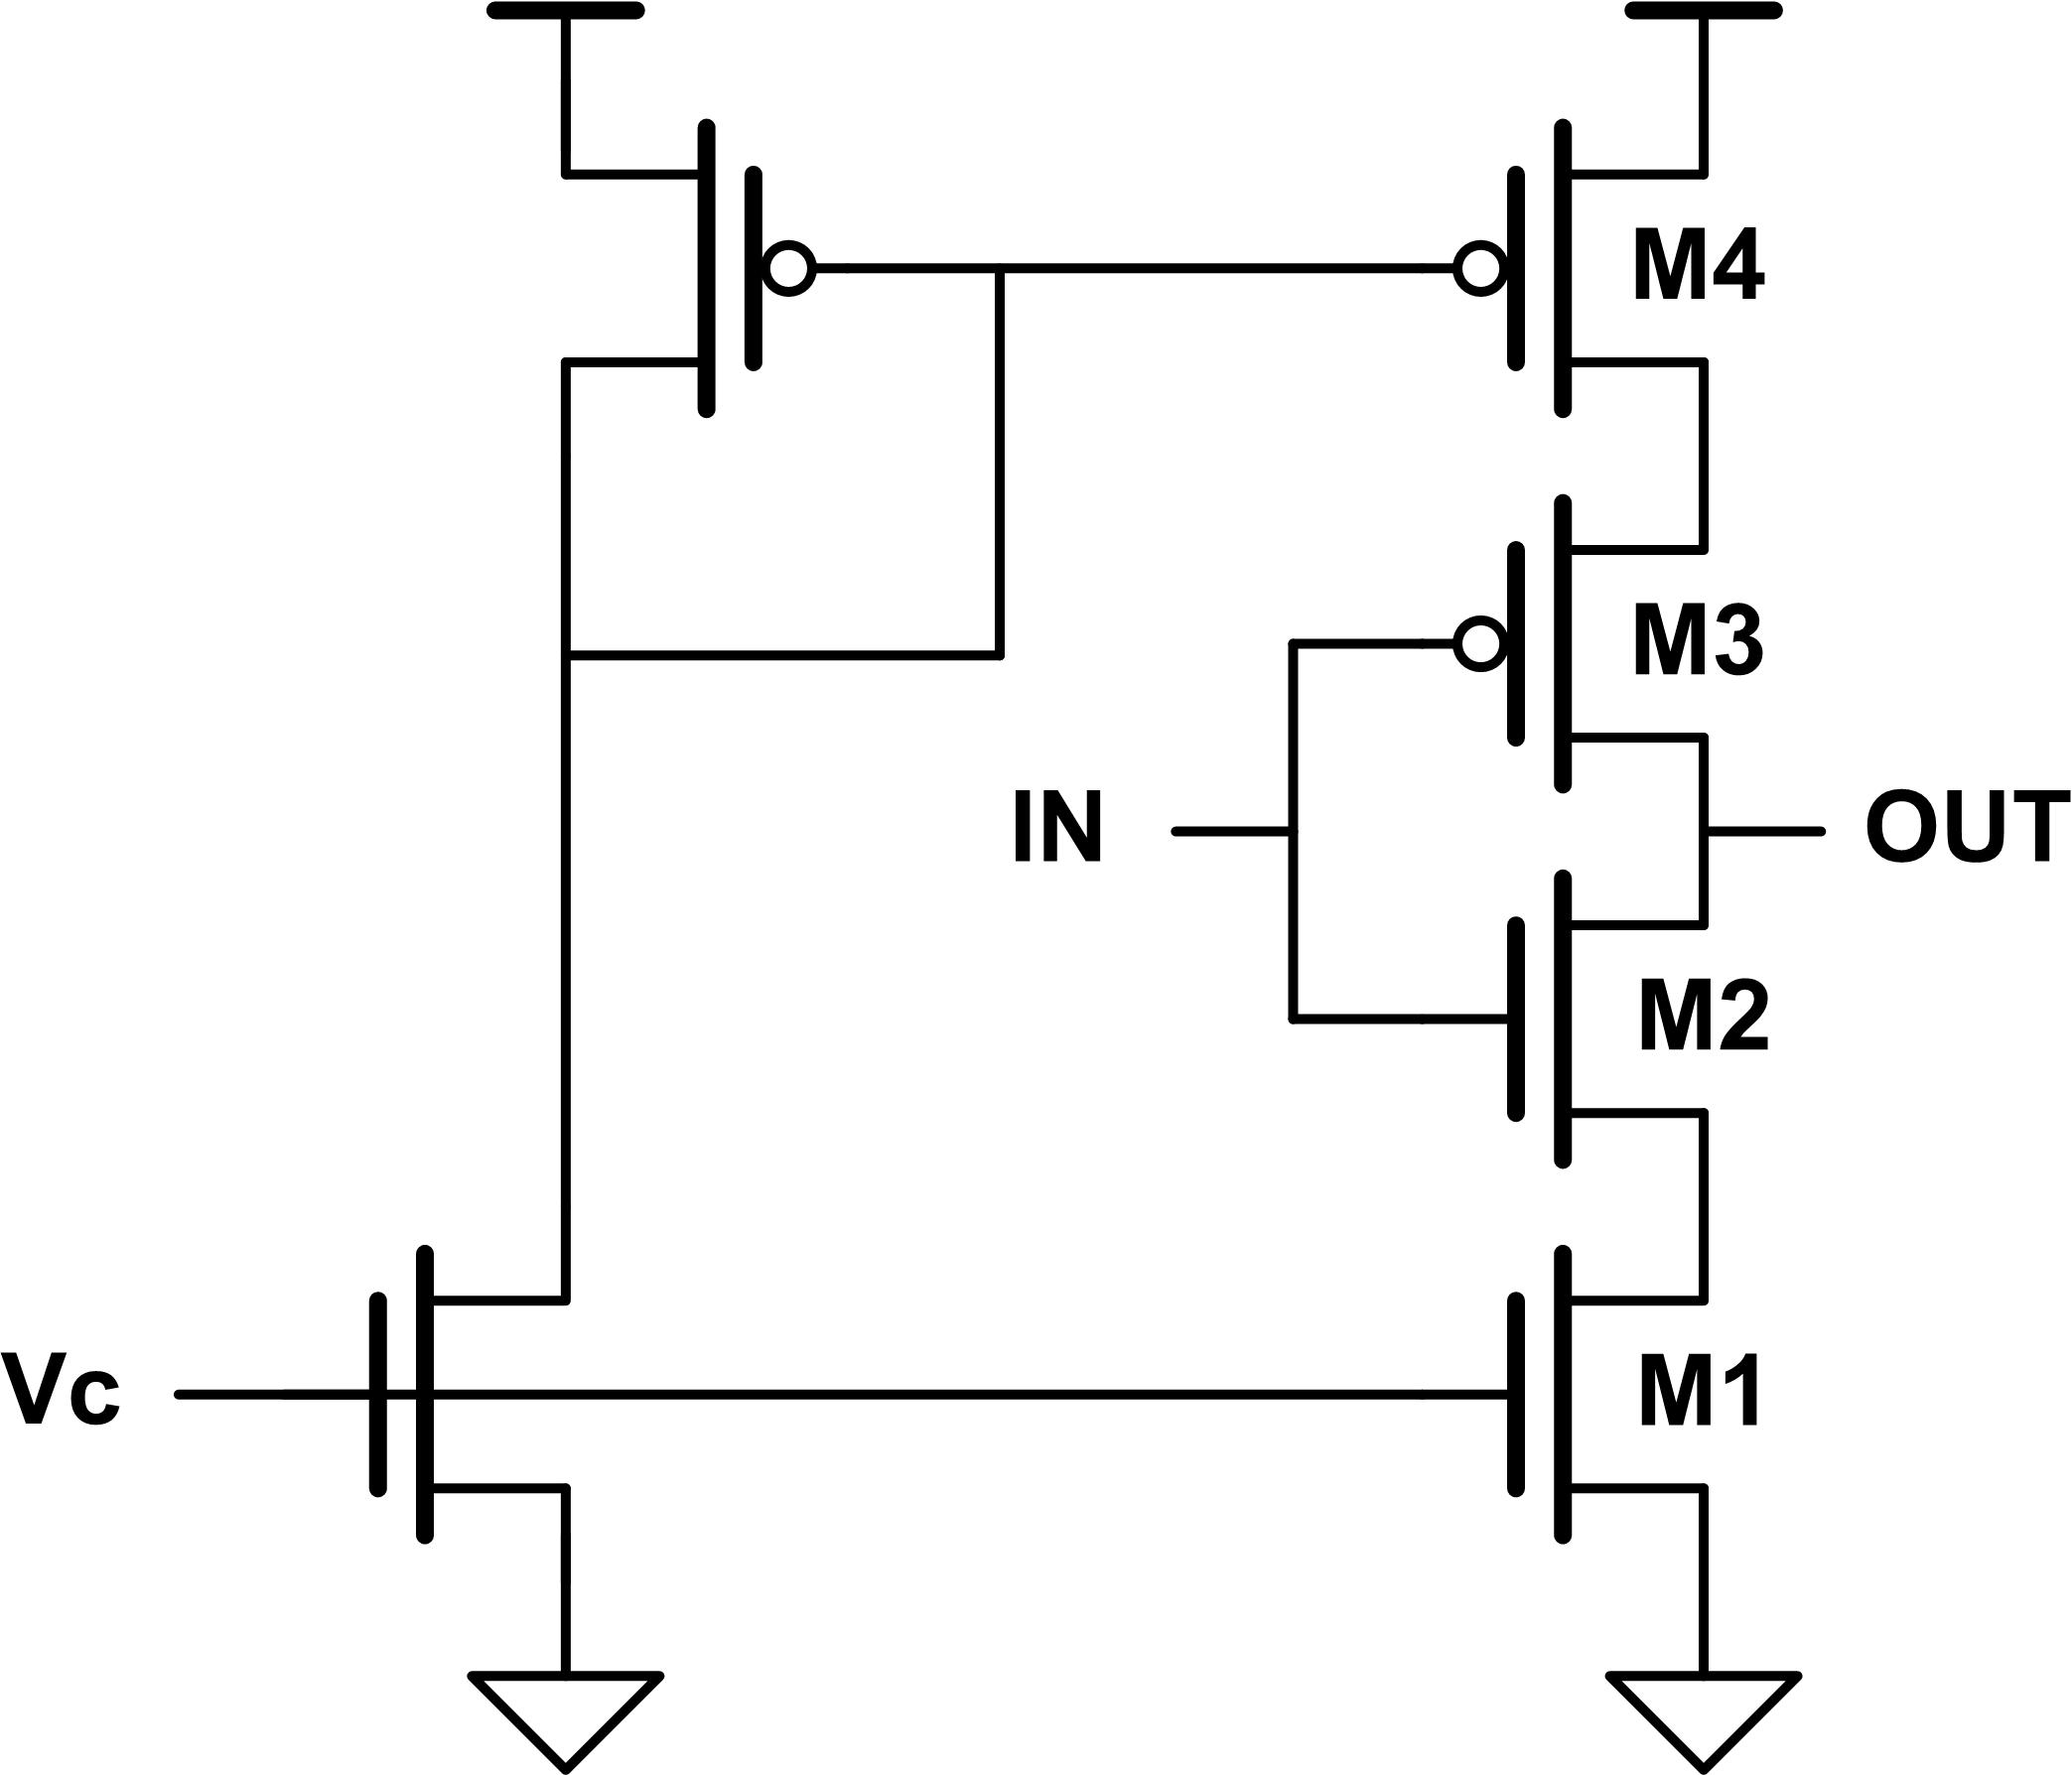
\includegraphics[scale=.5]{starver.jpg}
\caption{The current starver, which wraps one of the inverters to make the circuit tunable. \emph{Image courtesy of Brad Minch.}}
\label{starver}		
\end{figure} 		

\paragraph{Step Response}

When the circuit is initially powered on, each of the inverters' inputs are at a ``low'' state, since no voltage has yet propagated through the circuit.  Although each inverter has no bias voltage just yet, the source-drain voltages of the nMOS and pMOS transistors allows a very small amount of current to run pass through the inverters' channels. That small current causes the inverter output to have a small non-zero voltage. These, in turn, get amplified by the ring, and slowly these amplified oscillations grow into the full steady-state oscillation states.  These small voltages will initially vary somewhat by random chance, and so some voltages will come to dominate the others.  We saw this in our LTSpice simulation, as shown in Figure \ref{step}.

\begin{figure}[H]	
\centering			
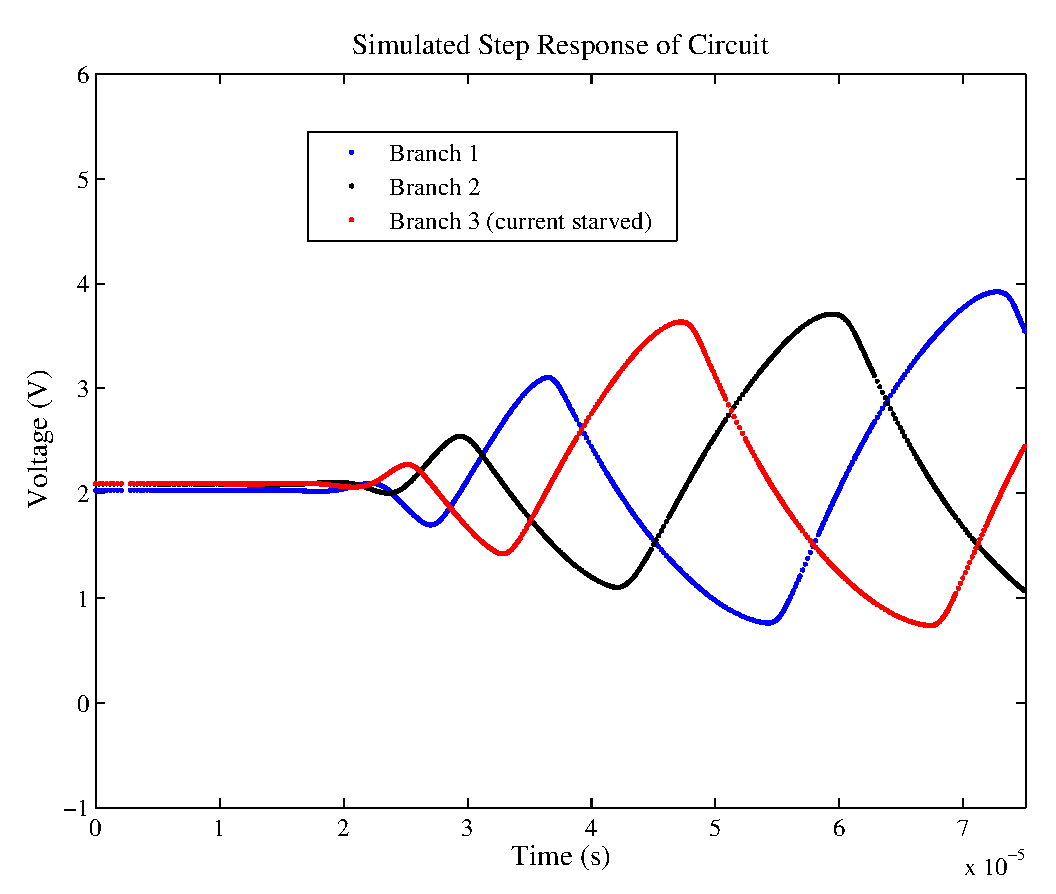
\includegraphics[scale=.6]{step.eps}
\caption{Simulated step response of the circuit. After making micro-oscillations for a few cycles, the circuit eventually saturates to a stable oscillation.}
\label{step}		
\end{figure} 	

\section*{Simulation Results}

To get an initial analysis of the circuit, we simulated a ring oscillator using LTSpice. The schematic that we used is shown in Figure \ref{schem}. The oscillor consists of 3 inverters, one of which is ``starved'' of current. The bias voltage determines the oscillation frequency by limiting the current to the third inverter. Takes longer to charge the capacitor, which limits the frequency. This current-starved third inverter sets the fundamental frequency of the oscillation. \\

Note: our convention is that \emph{branch 1}'s output goes into the input of \emph{branch 2}, the current-starved branch, which feeds into \emph{branch 3}.

\begin{figure}[H]
\centering
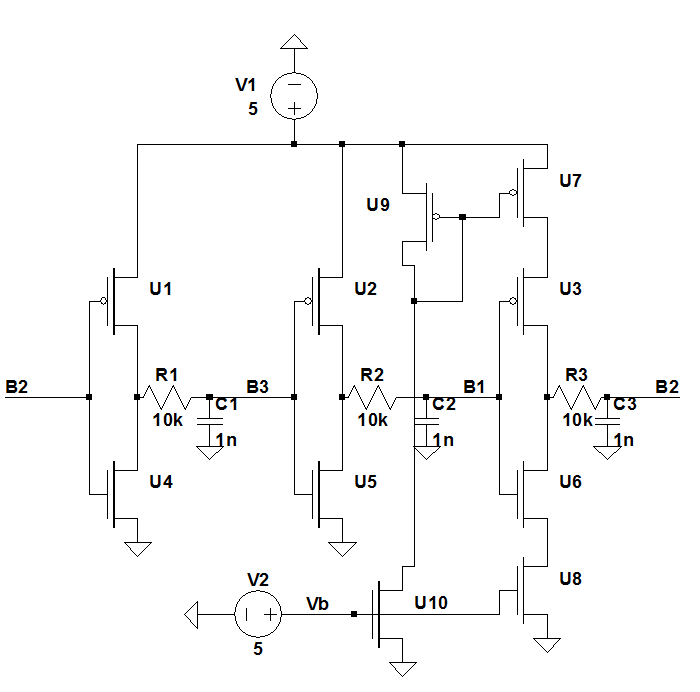
\includegraphics[scale=.5]{finalSchem2.png}
\caption{The schematic we used to simulate the oscillator in ltSpice}
\label{schem}
\end{figure}

The signal from the third inverter is amplified through each stage. This can be seen in figure \ref{lowBiasSigSim}. The bias transistor is in weak-moderate inversion, so it limits the output of the third inverter. The signal is amplified twice, until it is about rail-to-rail on branch 2. Figure \ref{highBiasSigSim} shows that when the bias transistor is in strong inversion, the gain isn't very high. Note that for both cases, the branches are out of phase with each other. This is because as one inverter output is high, the other two are either rising or falling. \\


\begin{figure}[H]
\centering
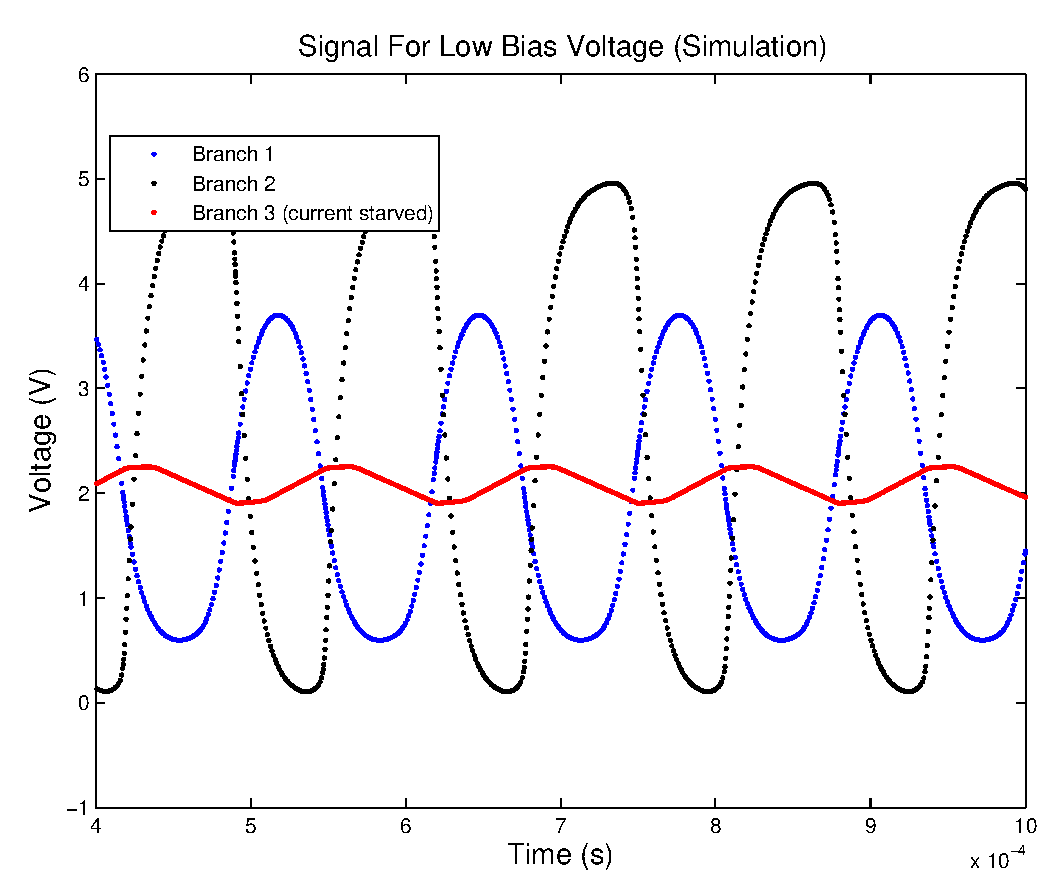
\includegraphics[scale=.7]{lowBiasSigSim.eps}
\caption{The output of each inverter for a low bias voltage.}
\label{lowBiasSigSim}
\end{figure}

\begin{figure}[H]
\centering
\includegraphics[scale=.7]{highBiasSigSim.eps}
\caption{The output of each inverter for a high bias voltage.}
\label{highBiasSigSim}
\end{figure}

Figure \ref{branch2DiffBiasSim} shows the differences in frequency between bias voltages. When the bias voltage is in moderate inversion, the current through the third inverter is limited. Any change of bias voltage in this region causes a significant change in frequency. We found the frequency by calculating the frequency of each signal in \texttt{MATLAB}. We then plotted frequency as a function of bias voltage, which is shown in figure \ref{biasFrequenciesSim}. Note that for strong inversion, the bias voltage has a relatively small effect on the frequency.

\begin{figure}[H]
\centering
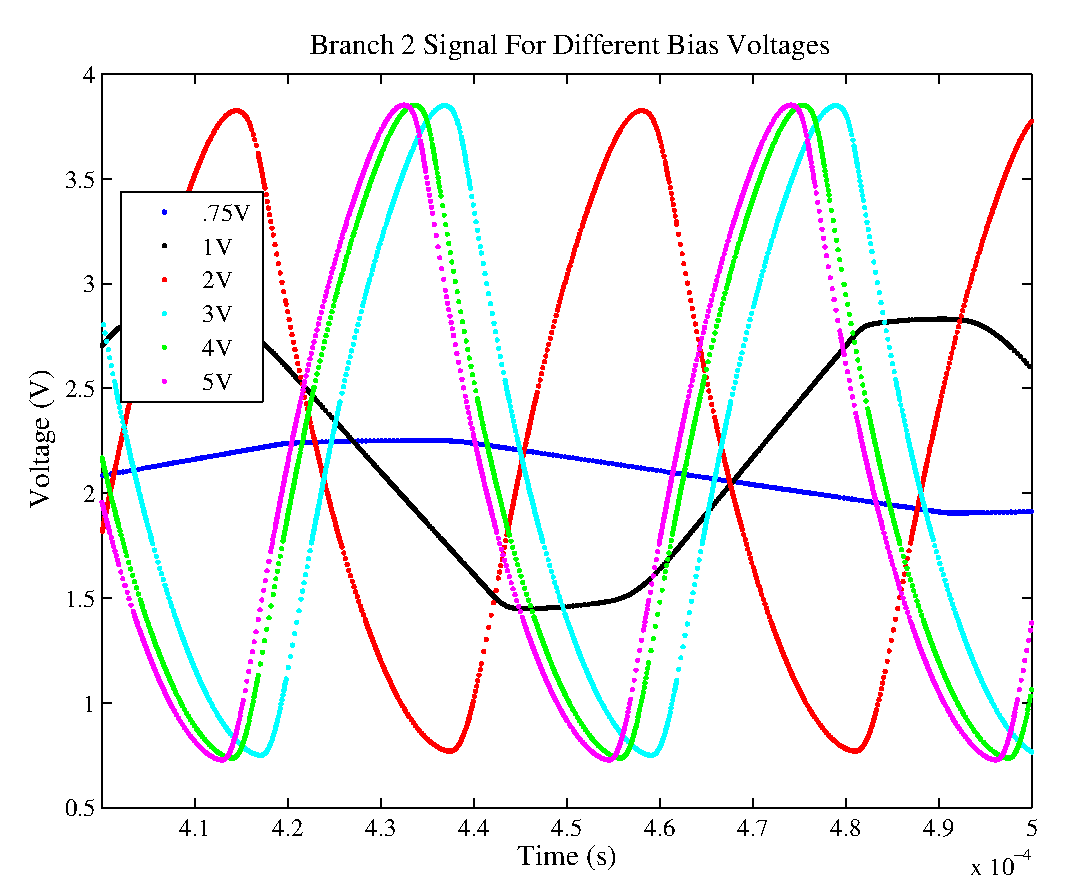
\includegraphics[scale=.7]{branch2DiffBiasSim.eps}
\caption{The output of the oscillator For different bias voltages. Note that increasing the bias voltage increases the frequency of the oscillator.}
\label{branch2DiffBiasSim}
\end{figure}


\begin{figure}[H]
\centering
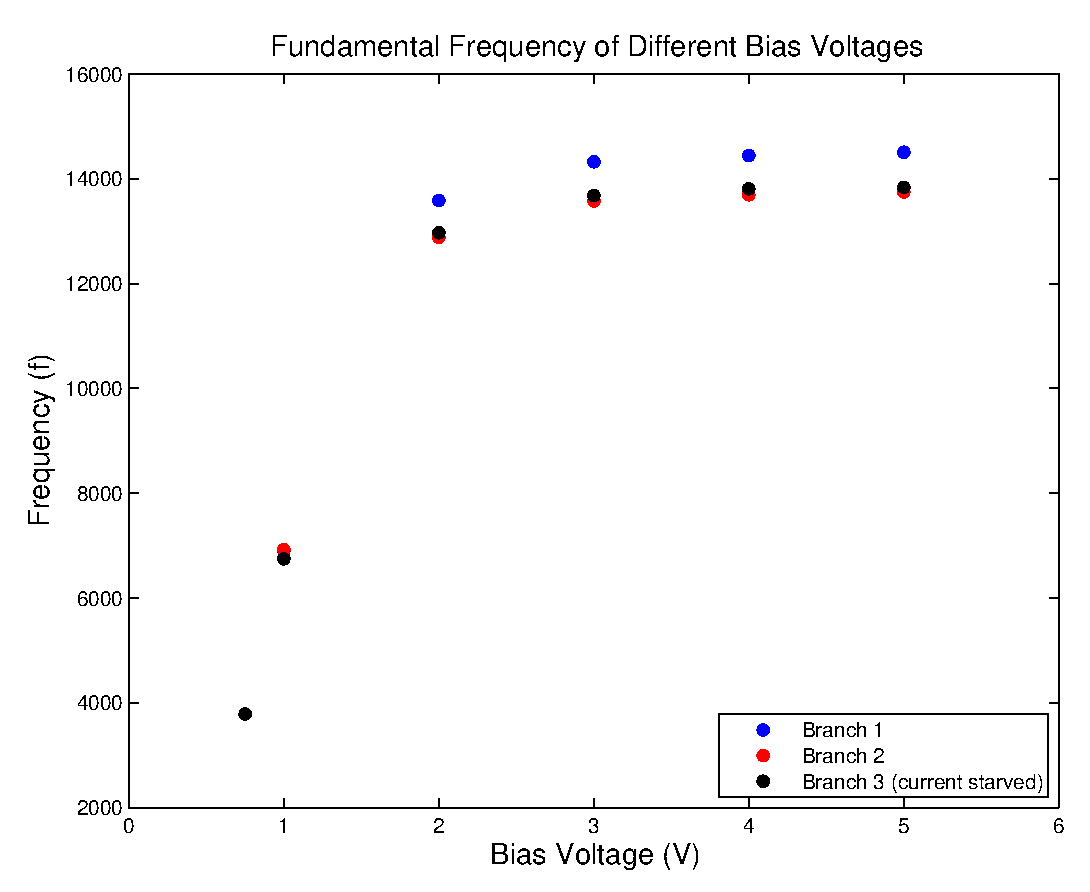
\includegraphics[scale=.7]{biasFrequenciesSim.eps}
\caption{The output frequency as a function of bias voltage. For a moderately inverted bias transistor, a change in bias voltage results in a large change in frequency, but this effect diminishes for larger bias voltages.}
\label{biasFrequenciesSim}
\end{figure}

\section*{Results}

We built the circuit and used an oscilloscope to view the oscillations.  We used 6 different bias voltages for the current starver to see how that affects the frequency of oscillation and measured the voltage on each branch of the circuit.

\subsection*{Time-Domain Analysis}

\subsubsection*{Large Bias Voltages}

If we apply a large bias voltage, 5V, to the current starver, we see that the three branches of the oscillator exhibit very similar waveforms.

\begin{figure}[H]
\centering
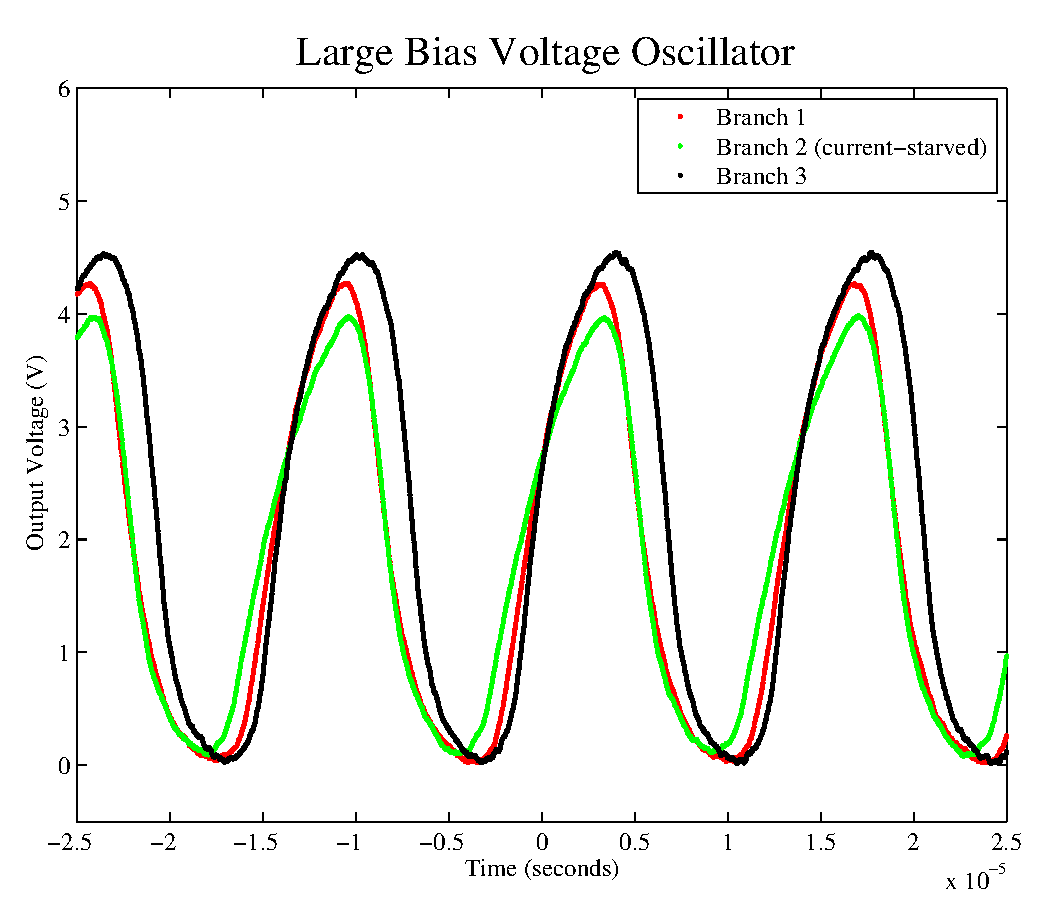
\includegraphics[scale=.6]{large_bias.eps}
\caption{Our circuit's response to a large bias voltage is a large-amplitude oscillation on every branch.  The current-starved branch has the smallest amplitude by the smallest amount, and the branch preceding it has the largest. }
\label{largeBias}
\end{figure}

The three branches all almost reach the rail.  The current starved branch, branch 2, is limited in its current, so its output is not able to reach a strong 0 or a strong 1.  The weak 1 or 0 being passed to the next branch, branch 3, is amplified to almost a strong 1 or strong 0, but, again, it does not quite reach that level.  That almost-strong 0 or 1 is able to get amplified closer to a strong bit when that gets passed to the third inverter, so it has the largest magnitude.

\subsubsection*{Small Bias Voltage}

If, instead, we apply a small bias voltage, .75V, to the bias transistor, we see that the system behaves very differently.  We chose .75V because it is close to that transistor's turn-on voltage (moderate inversion), and dropping below that point limited the current so severely that we were unable to see any waveforms on the oscilloscope.

\begin{figure}[H]
\centering
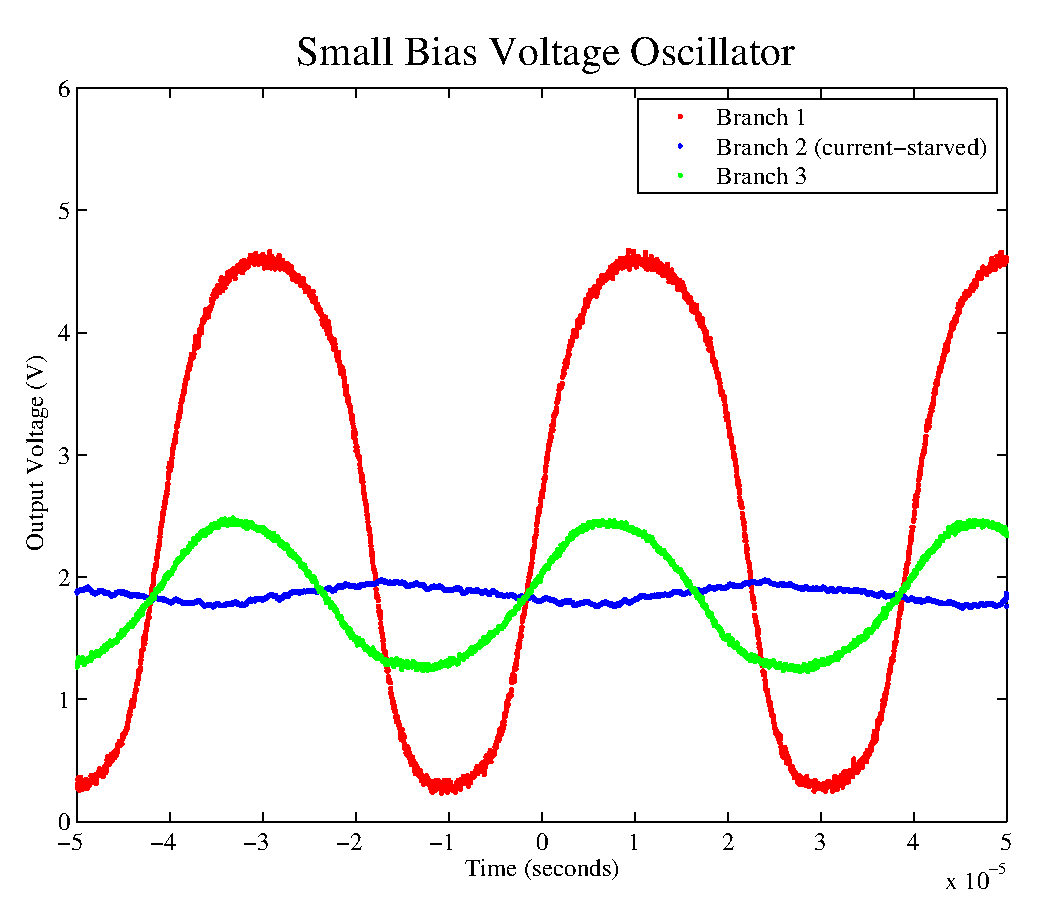
\includegraphics[scale=.6]{small_bias.eps}
\caption{The current-starved branch barely responds to the oscillations because there is so little current flowing through the circuit.  This gets amplified somewhat in the next branch, and almost fully amplified at the next inverter.}
\label{smallBias}
\end{figure}

This small bias voltage creates a remarkably different situation.  We see that the current-starved branch, branch 2, only oscillates very slightly and very linearly.  This is because its current is so small that the RC circuit between the branches does not saturate before the inverter's input reverses its direction, which makes the response look linear.  This small change in voltage, though, gets amplified by the next inverter, which turns it into a larger current and a larger output voltage at the next branch; this is manifested by a fuller oscillation, but with a low amplitude. This, in turn, creates an even-larger output voltage in the next inverter.

\subsubsection*{In-between Bias Voltage}

Unsurprisingly, applying a moderate voltage, 1V, such that the transistor is in strong inversion, produces results in between the strong and weak case.  The output voltage of the current-starved branch is small, and the output voltage quickly increases to close to the rail.

\begin{figure}[H]
\centering
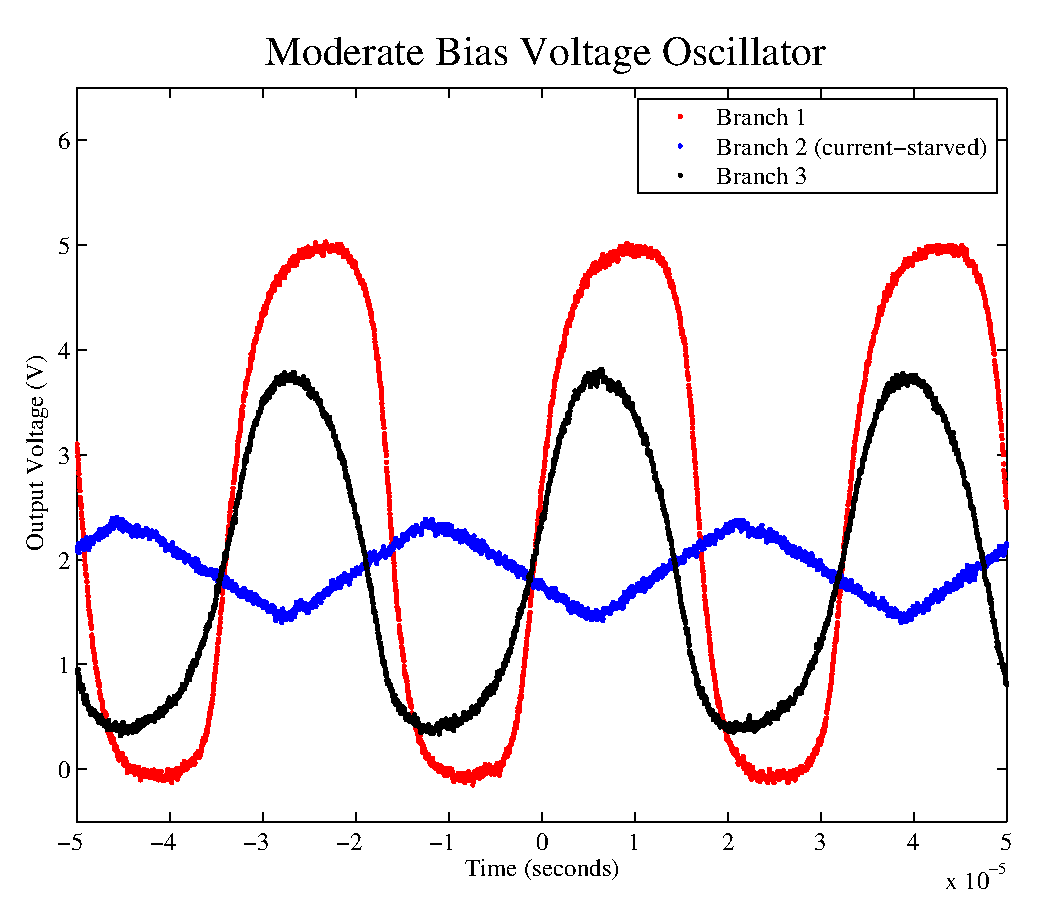
\includegraphics[scale=.6]{moderate_bias.eps}
\caption{The moderate-bias response of the circuit. }
\label{moderateBias}
\end{figure}

\subsection*{Frequency Analysis}

At the heart of this project was the desire to make a tunable oscillator. As a result, being able to change the frequency by tweaking a voltage is interesting and useful.  For example, we imagine that many applications required two frequencies to match very precisely, and being able to make small changes to the frequency just by changing the bias voltage could be used to make those frequencies match.  We saw above that tuning the bias voltage changes the shape of the waves and their amplitudes, but, more importantly, it changes their frequency as well (since the RC circuits take longer to charge).  This can be seen visually in Figure \ref{branch}, where the increasing bias voltages causes the resulting waves to increase in frequency.

\begin{figure}[H]
\centering
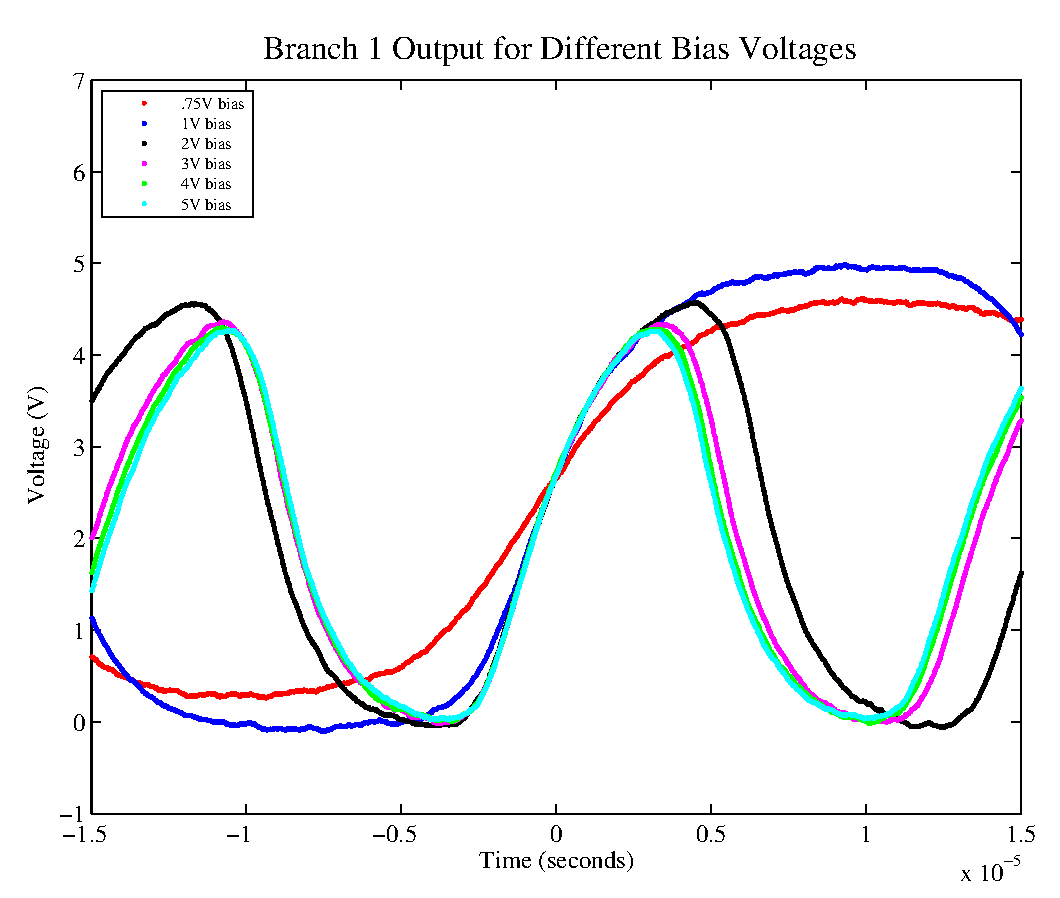
\includegraphics[scale=.6]{b1_out.eps}
\caption{A time-domain view of the changing frequencies of the ring oscillator. With increasing bias voltage, the waves shrink together, corresponding to an increase in frequency.}
\label{branch}
\end{figure}

We used \texttt{MATLAB} to calculate the frequency of these waves as a function of input voltage.  We found that each branch had nearly identical measured voltage for a given bias voltage, which makes sense given how each branch depends on every other.  This can be seen in Figure \ref{freqs}.

\begin{figure}[H]
\centering
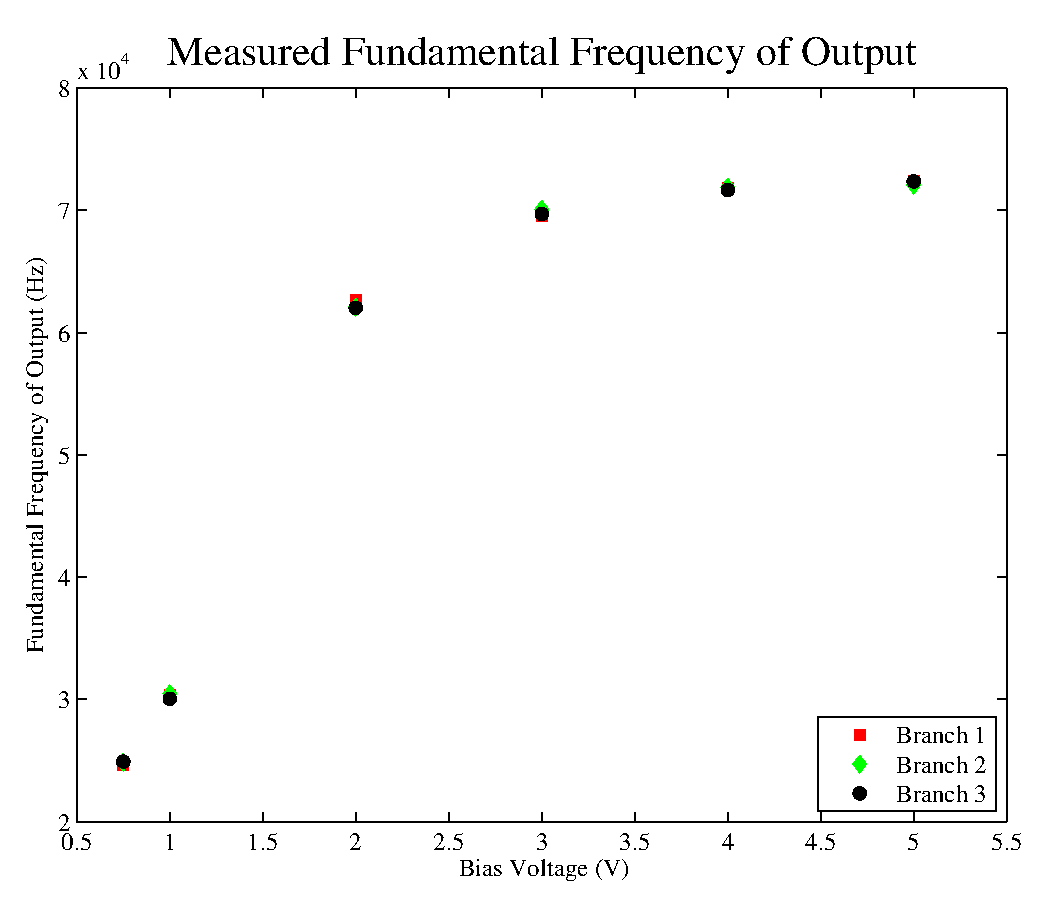
\includegraphics[scale=.5]{freqs.eps}
\caption{The frequency of the ring oscillator depends strongly on bias voltage for voltages near the turn-on voltage of the bias transistor, then shallows out near the rails.}
\label{freqs}
\end{figure}

The change in frequency is more pronounced for small bias voltages, and then flattens out as the voltages increase towards the rail.  This is because changes in voltage near the turn-on voltage causes a roughly exponential increase in current, while further from the turn-on voltage, the current increases more slowly (quadratically).  

\section{Comparison}

\end{document}